\documentclass[11pt]{article}
\usepackage[review]{acl}
\usepackage{times,latexsym}
\usepackage[T1]{fontenc}
\usepackage[utf8]{inputenc}
\usepackage{microtype,inconsolata}
\usepackage{graphicx,booktabs,multirow,amsmath,amssymb}
\usepackage{tikz,pgfplots}
\usetikzlibrary{arrows.meta,positioning,calc,fit,backgrounds}
\usepgfplotslibrary{groupplots}
\pgfplotsset{compat=1.18}
\definecolor{ink}{HTML}{20334D}
\definecolor{teal}{HTML}{087E8B}
\definecolor{orange}{HTML}{CC702D}
\definecolor{bluegray}{HTML}{5C6E91}
\definecolor{mist}{HTML}{EDF1F5}
\newcommand{\method}{ReFit}
\newcommand{\stat}[2]{\begin{tabular}[c]{@{}c@{}}#1\\[-2pt]{\scriptsize[#2]}\end{tabular}}
\newcommand{\ci}[2]{[#1,\,#2]}
\newcommand{\KL}{\operatorname{KL}}
\newcommand{\argmax}{\operatorname*{arg\,max}}
\hypersetup{pdftitle={Mind the Interface: Repairing Speculative Decoding after Target Model Post-Training},pdfauthor={Anonymous},pdfsubject={Working research draft; measured pilot snapshot, October 10, 2026}}
\title{Mind the Interface: Repairing Speculative Decoding\\after Target Model Post-Training}
\author{Anonymous ACL submission}
\begin{document}
\maketitle

\begin{abstract}
Target-conditioned drafters such as EAGLE-3 accelerate language models by reading the target's hidden states, but this tight coupling becomes a liability when the target is post-trained. We show that reusing a family drafter can lose substantial acceptance on reasoning and alternative post-training trajectories, under both EAGLE-3 and DFlash. We trace the loss to changes in both the target's token policy and the feature interface through which the drafter reads the target. We introduce \method{}, a training-set-free repair procedure that elicits responses from the updated target and refits this existing interface while leaving the target, draft architecture, and verification rule unchanged. With 16,000 public prompts, interface repair recovers 59.9\% of the acceptance-length gap between reuse and a dedicated drafter on R1-Distill-Llama-8B across three seeds; full warm-start repair recovers 71.7\%. The repairs raise measured A40 batch-1 speedup from $1.31\times$ under reuse to $1.74\times$ and $1.83\times$, respectively, while the dedicated drafter reaches $2.05\times$. Gains transfer to Nemotron-Nano-8B and to a DFlash pilot. These results make interface repair a practical way to preserve speculative decoding as target models change.
\end{abstract}

\section{Introduction}
Speculative decoding accelerates language-model generation without changing its output: a small drafter proposes several tokens, and the target verifies them in one forward pass \citep{leviathan2023,chen2023}. Its speed depends on how many proposals the target accepts. The strongest drafters increasingly condition on the target's own hidden states. EAGLE-3 fuses features from three target layers, while DFlash uses target features to predict a block in parallel \citep{eagle32025,dflash2026}. This coupling makes drafting accurate and cheap, but it also binds the drafter to the checkpoint that supplied its training features and token supervision.

Open target models do not remain fixed. A popular release spawns reasoning distillations, supervised fine-tunes, preference-optimized variants, merges, and reinforcement-learning checkpoints. A compatible family drafter may exist for the official instruction model, while no dedicated drafter exists for the post-trained target and the target's original training data are unavailable. Training a full drafter for every release defeats much of the practical value of an open model ecosystem. The resulting question is simple: when a target changes, can we retain what its family drafter already knows?

We first measure when reuse succeeds. In a paired frozen-harness study of public Llama and Qwen checkpoints, sampled direct-child on-policy RL models retain nearly all of the family drafter's first-token acceptance. Reasoning distillations and other post-training trajectories can lose far more, in both autoregressive EAGLE-3 and block-diffusion DFlash. R1-Distill-Llama-8B, for example, reaches only $\tau=1.76$ with a reused family drafter, versus $2.85$ with a dedicated EAGLE-3 drafter. Because reasoning models often generate long answers, this loss appears where speculative acceleration is especially valuable.

\begin{figure*}[t]
\centering
\resizebox{\textwidth}{!}{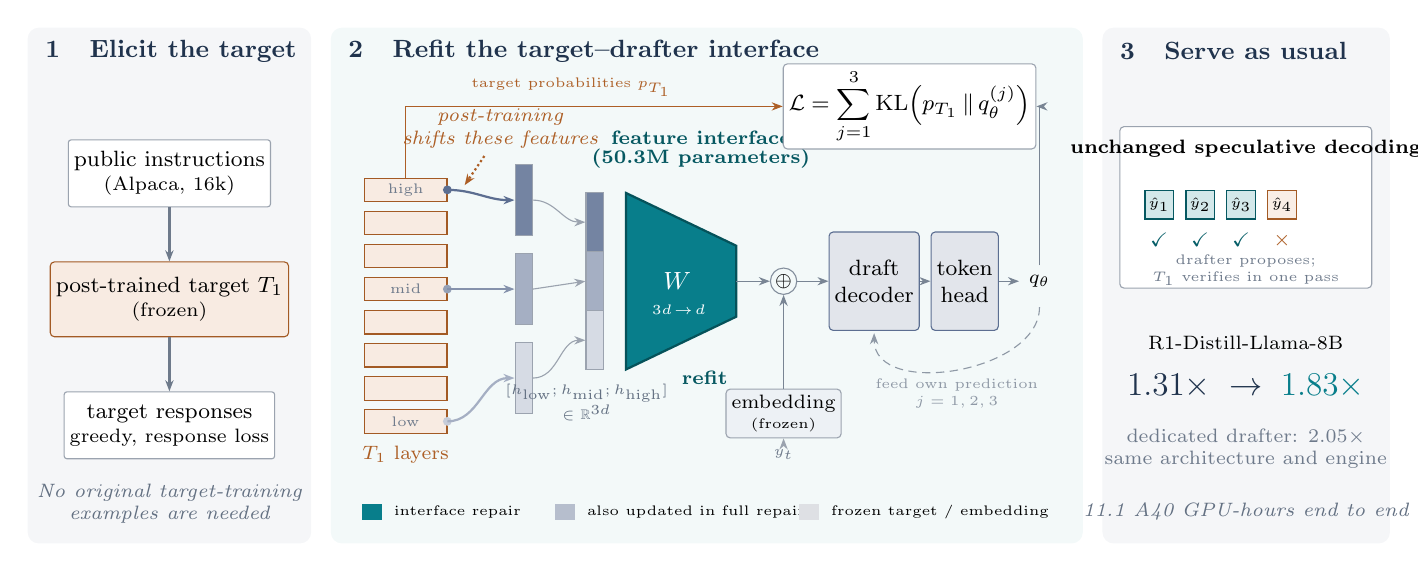
\begin{tikzpicture}[
  font=\footnotesize, >={Stealth[length=4pt]},
  doc/.style={draw=ink!45,fill=white,rounded corners=1pt,minimum width=2.5cm,minimum height=.85cm,align=center,inner sep=2pt},
  blk/.style={draw=ink!45,rounded corners=1.5pt,align=center,inner sep=2pt},
  layer/.style={draw=orange!80!black,fill=orange!14,minimum width=1.05cm,minimum height=.30cm,inner sep=0pt},
  hdr/.style={font=\small\bfseries,anchor=west,text=ink},
  feat/.style={draw=ink!45,minimum width=.22cm,minimum height=.9cm,inner sep=0pt},
  note/.style={font=\scriptsize\itshape,text=ink!70,align=center}]
\path[use as bounding box] (-.25,-1.55) rectangle (17.05,5.0);
\fill[bluegray!6,rounded corners=4pt] (-.25,-1.55) rectangle (3.35,5.0);
\fill[teal!5,rounded corners=4pt] (3.6,-1.55) rectangle (13.15,5.0);
\fill[bluegray!6,rounded corners=4pt] (13.4,-1.55) rectangle (17.05,5.0);
\node[hdr] at (-.15,4.7) {1\quad Elicit the target};
\node[hdr] at (3.7,4.7) {2\quad Refit the target--drafter interface};
\node[hdr] at (13.5,4.7) {3\quad Serve as usual};

\node[doc] (prompts) at (1.55,3.15) {public instructions\\[-1pt]\scriptsize(Alpaca, 16k)};
\node[blk,fill=orange!14,draw=orange!80!black,minimum width=2.5cm,minimum height=.95cm] (tgt) at (1.55,1.55) {post-trained target $T_1$\\[-1pt]\scriptsize(frozen)};
\node[doc] (resp) at (1.55,-.05) {target responses\\[-1pt]\scriptsize greedy, response loss};
\draw[->,thick,ink!65] (prompts)--(tgt); \draw[->,thick,ink!65] (tgt)--(resp);
\node[note] at (1.55,-1.05) {No original target-training\\examples are needed};

\foreach \i in {0,...,7}{\node[layer] (L\i) at (4.55,0+.42*\i) {};}
\node[font=\scriptsize,text=orange!85!black] at (4.55,-.42) {$T_1$ layers};
\node[font=\tiny,text=ink!65] at (4.55,0) {low}; \node[font=\tiny,text=ink!65] at (4.55,1.68) {mid}; \node[font=\tiny,text=ink!65] at (4.55,2.94) {high};
\coordinate (tapL) at (5.08,0); \coordinate (tapM) at (5.08,1.68); \coordinate (tapH) at (5.08,2.94);
\foreach \t/\c in {tapL/bluegray!35,tapM/bluegray!65,tapH/bluegray}{\fill[\c] (\t) circle (1.6pt);}
\node[feat,fill=bluegray!25] (fl) at (6.05,.55) {}; \node[feat,fill=bluegray!55] (fm) at (6.05,1.68) {}; \node[feat,fill=bluegray!85] (fh) at (6.05,2.81) {};
\draw[->,bluegray!55,thick] (tapL) to[out=0,in=180] (fl.west); \draw[->,bluegray!75,thick] (tapM)--(fm.west); \draw[->,bluegray,thick] (tapH) to[out=0,in=180] (fh.west);
\node[feat,minimum height=.75cm,fill=bluegray!25] (c1) at (6.95,1.03) {}; \node[feat,minimum height=.75cm,fill=bluegray!55] (c2) at (6.95,1.78) {}; \node[feat,minimum height=.75cm,fill=bluegray!85] (c3) at (6.95,2.53) {};
\draw[->,ink!45] (fl.east) to[out=0,in=180] (c1.west); \draw[->,ink!45] (fm.east)--(c2.west); \draw[->,ink!45] (fh.east) to[out=0,in=180] (c3.west);
\node[font=\tiny,align=center,anchor=north,text=ink!70] at (6.85,.6) {$[h_{\rm low};h_{\rm mid};h_{\rm high}]$\\$\in\mathbb{R}^{3d}$};
\node[note,text=orange!85!black,anchor=south] at (5.75,3.35) {post-training\\shifts these features}; \draw[->,orange!85!black,densely dotted,thick] (5.55,3.37)--(5.3,3.0);

\fill[teal,draw=teal!65!black,thick] (7.35,.66)--(8.75,1.33)--(8.75,2.23)--(7.35,2.9)--cycle;
\node[font=\small\bfseries,text=white] at (8.0,1.78) {$W$}; \node[font=\tiny,text=white] at (8.02,1.42) {$3d\!\to\!d$};
\node[font=\scriptsize\bfseries,text=teal!70!black,align=center] at (8.3,3.45) {feature interface\\[-1pt]\scriptsize(50.3M parameters)}; \node[font=\scriptsize\bfseries,text=teal!70!black] at (8.35,.55) {refit};
\node[blk,fill=mist,minimum width=1.15cm,minimum height=.5cm] (emb) at (9.35,.1) {\scriptsize embedding\\[-2pt]\tiny(frozen)};
\node[circle,draw=ink!55,inner sep=.5pt,font=\scriptsize] (plus) at (9.35,1.78) {$\oplus$};
\draw[->,ink!60] (8.75,1.78)--(plus.west); \draw[->,ink!60] (emb.north)--(plus.south); \node[font=\tiny,text=ink!65] at (9.35,-.42) {$y_t$}; \draw[->,ink!45] (9.35,-.3)--(emb.south);
\node[blk,fill=bluegray!18,draw=bluegray,minimum width=1.05cm,minimum height=1.25cm] (dec) at (10.5,1.78) {draft\\decoder};
\node[blk,fill=bluegray!18,draw=bluegray,minimum width=.85cm,minimum height=1.25cm] (head) at (11.65,1.78) {token\\head};
\draw[->,ink!60] (plus.east)--(dec.west); \draw[->,ink!60] (dec.east)--(head.west); \node[font=\scriptsize] (q) at (12.6,1.78) {$q_\theta$}; \draw[->,ink!60] (head.east)--(q.west);
\draw[->,ink!50,densely dashed] (12.6,1.45) to[out=-90,in=-90,looseness=1] node[pos=.5,below,font=\tiny,align=center] {feed own prediction\\$j=1,2,3$} (10.5,1.12);
\node[blk,fill=white,minimum height=.55cm] (loss) at (10.95,4.0) {$\displaystyle \mathcal L=\sum_{j=1}^{3}\KL\!\left(p_{T_1}\,\|\,q_\theta^{(j)}\right)$};
\draw[->,orange!85!black] (L7.north)|-node[pos=.72,above,font=\tiny] {target probabilities $p_{T_1}$}(loss.west); \draw[->,ink!60] (q.north)|-(loss.east);
\fill[teal] (4,-1.25) rectangle (4.25,-1.05); \node[font=\tiny,anchor=west] at (4.28,-1.15) {interface repair};
\fill[bluegray!45] (6.45,-1.25) rectangle (6.7,-1.05); \node[font=\tiny,anchor=west] at (6.73,-1.15) {also updated in full repair};
\fill[ink!15] (9.55,-1.25) rectangle (9.8,-1.05); \node[font=\tiny,anchor=west] at (9.83,-1.15) {frozen target / embedding};

\node[blk,fill=white,minimum width=3.2cm,minimum height=2.05cm,anchor=north] (srv) at (15.22,3.75) {}; \node[font=\scriptsize\bfseries,anchor=north] at (15.22,3.7) {unchanged speculative decoding};
\foreach \j/\ok in {0/1,1/1,2/1,3/0}{\pgfmathsetmacro{\xx}{14.12+.52*\j}\ifnum\ok=1\node[draw=teal!70!black,fill=teal!18,minimum size=.36cm,inner sep=0pt,font=\tiny] at (\xx,2.75) {$\hat y_{\the\numexpr\j+1\relax}$};\node[font=\scriptsize,text=teal!75!black] at (\xx,2.3) {$\checkmark$};\else\node[draw=orange!80!black,fill=orange!12,minimum size=.36cm,inner sep=0pt,font=\tiny] at (\xx,2.75) {$\hat y_{\the\numexpr\j+1\relax}$};\node[font=\scriptsize,text=orange!85!black] at (\xx,2.3) {$\times$};\fi}
\node[font=\tiny,text=ink!65,align=center] at (15.22,1.92) {drafter proposes;\\$T_1$ verifies in one pass};
\node[font=\scriptsize,align=center] at (15.22,1.0) {R1-Distill-Llama-8B}; \node[font=\large\bfseries,align=center,text=ink] at (15.22,.45) {$1.31\times\;\rightarrow\;\textcolor{teal}{1.83\times}$};
\node[font=\scriptsize,text=ink!65,align=center] at (15.22,-.35) {dedicated drafter: $2.05\times$\\same architecture and engine}; \node[note] at (15.22,-1.15) {11.1 A40 GPU-hours end to end};
\end{tikzpicture}
}
\caption{\textbf{\method{} teaches an existing drafter to read a changed target.} The target answers public instructions, then supplies hidden states and token probabilities under teacher forcing. Interface repair updates only the existing feature projection (teal); full repair also updates the draft decoder and head (blue). The target remains frozen. The repaired drafter keeps its architecture and is served by the same draft-and-verify engine.}
\label{fig:hero}
\end{figure*}

The failure is concentrated enough to repair. Post-training changes both the desired next token and the target features from which a target-conditioned drafter predicts it. A fixed-prefix crossover exchanges feature sources and verifier policies while holding text constant; it detects both effects. Component-matched adaptation then shows that the dense projection from target features into the draft decoder carries most of the recoverable gain. This projection is therefore the natural place to teach a released drafter how to read its new target.

We introduce \method{}, a repair procedure that uses the new target's own responses to public instructions. It keeps the target fixed and retains the released drafter's architecture, token support, and native training objective. The primary variant updates only the projection from target hidden states into the draft decoder. A full warm-start variant uses the same data and budget to update the remaining trainable draft components as well. Neither requires the target's original post-training corpus or a new serving architecture.

The tradeoff is concrete. On R1-Distill-Llama-8B, interface repair increases first-position acceptance from 43.0\% to 62.6\% and recovers 59.9\% of the gap between reuse and a dedicated R1 drafter. Full repair reaches 65.0\% acceptance and 71.7\% gap recovery. Interface repair updates 50.3 million parameters rather than 424.7 million, while full repair offers greater acceptance at a similar measured training time. Both produce real latency improvements, including on Nemotron, for which we have no dedicated-drafter reference.

Our contributions connect diagnosis to deployment. We present a lineage-aware study of family-drafter compatibility across public checkpoints; localize the repair opportunity with a controlled feature--policy crossover and component-matched adaptations; and introduce an interface-first repair evaluated with paired acceptance, dedicated-drafter gap recovery, measured compute, and wall-clock speed. Together, these results show how to preserve a speculative drafter after the target model changes.



\section{When Does a Family Drafter Need Repair?}
\label{sec:study}
Let $T_0$ be the target for which a family drafter $D_0$ was trained, and let $T_1$ be the model we wish to serve. $T_1$ can be a direct post-trained child of $T_0$, a sibling trained from the same pretrained base, or a composite model. We study the transfer from $(T_0,D_0)$ to $(T_1,D_0)$ without retraining either target. The sibling case is especially relevant for reasoning distillation: the pretrained ancestor can be shared even when the instruction model is not the new target's immediate parent.

\subsection{Paired compatibility measurements}
We use first-position conditional acceptance, $p_1$, to measure immediate draft--target agreement, and macro acceptance length, $\tau$, to measure accepted progress per speculative iteration. For query $i$ with $N_i$ speculative iterations and $a_{it}$ accepted draft tokens in iteration $t$,
\begin{equation}
\tau_i = 1 + \frac{1}{N_i}\sum_{t=1}^{N_i} a_{it},
\qquad \tau=\frac{1}{n}\sum_{i=1}^{n}\tau_i.
\label{eq:tau}
\end{equation}
The added one includes the target's bonus or replacement token. We likewise average $p_1$ over queries. Conditional acceptance at depth $j$ considers iterations that reached and proposed that depth. This separates immediate compatibility from the length of the full accepted block.

To measure transfer, we evaluate $T_0$ and $T_1$ on identical token IDs rendered with $T_1$'s chat template. Retention is the ratio $p_1(T_1,D_0)/p_1(T_0,D_0)$. Using the new target's rendered inputs in both arms prevents template changes from masquerading as weight changes. We report output lengths alongside $\tau$, because post-training also changes how long and in what style the target responds. First-position retention provides the headline comparison without relying on deep accepted blocks.

Our focused frozen-harness panel contains 21 eligible post-trained checkpoints from the Llama and Qwen families, each evaluated with EAGLE-3 and DFlash on 128 SPEED queries. We record lineage separately from training history using model-card evidence. Figure~\ref{fig:retention} summarizes three groups with multiple checkpoints. Direct-child on-policy RL checkpoints retain mean $p_1$ of 0.986 for EAGLE-3 and 0.990 for DFlash. Sibling models with SFT and teacher distillation retain 0.898 and 0.862, respectively. Nemotron, whose history combines SFT, RL, and merging, retains 0.696 and 0.708. These descriptive differences motivate targeted repair rather than automatic retraining of every new checkpoint.

\begin{figure}[t]
\centering
% Source: reports/P1-typed-population-20261008.md, hierarchical checkpoint/query CIs.
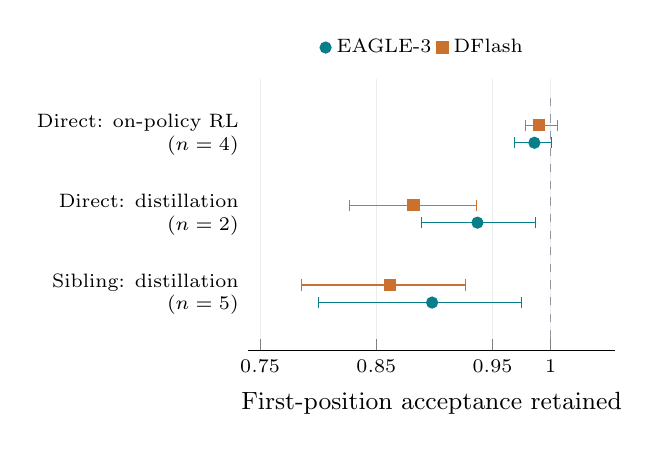
\begin{tikzpicture}
\begin{axis}[scale only axis,width=4.65cm,height=3.45cm,xmin=.74,xmax=1.055,ymin=.3,ymax=3.7,
 xlabel={First-position acceptance retained},ytick={1,2,3},
 yticklabels={Sibling: distillation\\($n=5$),Direct: distillation\\($n=2$),Direct: on-policy RL\\($n=4$)},
 yticklabel style={font=\scriptsize,align=right},
 xtick={.75,.85,.95,1.0},tick label style={font=\scriptsize},xlabel style={font=\small},
 axis x line*=bottom,axis y line*=left,y axis line style={draw=none},ytick style={draw=none},xmajorgrids,grid style={gray!15},
 legend style={at={(.48,1.04)},anchor=south,legend columns=2,draw=none,font=\scriptsize},
 clip=false]
\draw[dashed,ink!50] (axis cs:1,.45)--(axis cs:1,3.48);
\addplot+[only marks,mark=*,color=teal,mark options={fill=teal,draw=teal},error bars/.cd,x dir=both,x explicit]
 coordinates {(.898,.9) +=(.077,0) -=(.098,0) (.937,1.9) +=(.050,0) -=(.048,0) (.986,2.9) +=(.015,0) -=(.017,0)};
\addlegendentry{EAGLE-3}
\addplot+[only marks,mark=square*,color=orange,mark options={fill=orange,draw=orange},error bars/.cd,x dir=both,x explicit]
 coordinates {(.862,1.12) +=(.065,0) -=(.076,0) (.882,2.12) +=(.054,0) -=(.055,0) (.990,3.12) +=(.016,0) -=(.012,0)};
\addlegendentry{DFlash}
\end{axis}
\end{tikzpicture}

\caption{\textbf{Compatibility depends on the target's post-training trajectory.} Mean $p_1$ retention on SPEED-128 for groups with multiple checkpoints; bars are 95\% hierarchical checkpoint-and-query intervals. ``Direct'' and ``sibling'' denote lineage relative to the family drafter's target. Distillation groups also use SFT. The dashed line denotes unchanged acceptance.}
\label{fig:retention}
\end{figure}

\subsection{Separating feature and policy changes}
\label{sec:crossover}
A lower acceptance rate on a reasoning model can reflect a different generated context, different target features on that context, or a different next-token policy. We isolate the latter two with a fixed-prefix crossover. For each saved token prefix $x$, we feed either $T_0$'s or $T_1$'s hidden states to the frozen family drafter, and compare its first draft token against either target's greedy next token. Let $a_{uv}$ be agreement with feature source $u$ and verifier $v$, where $u,v\in\{0,1\}$. All four conditions use exactly the same prefix.

The averaged feature-source and verifier-policy effects are
\begin{align}
E_h &= \tfrac12[(a_{10}-a_{00})+(a_{11}-a_{01})],\\
E_p &= \tfrac12[(a_{01}-a_{00})+(a_{11}-a_{10})].
\end{align}
We also retain their interaction, $a_{11}-a_{10}-a_{01}+a_{00}$. This is a teacher-forced diagnostic, distinct from online speculative acceptance.

On 64 target-generated contexts per model, R1-Llama has a feature-source effect of $-2.0$ percentage points (95\% CI $[-2.5,-1.4]$) and a verifier-policy effect of $-3.0$ points ($[-3.5,-2.6]$). For Nemotron, these effects are $-6.9$ ($[-7.7,-6.2]$) and $-3.7$ ($[-4.3,-3.1]$) points. Positive interactions show that the two changes are coupled. These effects motivate learning the projection against the new target's token supervision, so that it can respond to changed features and their changed relationship to the verifier policy.

\section{\method{}: Interface-First Drafter Repair}
\label{sec:method}
Figure~\ref{fig:hero} gives the complete procedure. \method{} starts from a released family drafter and adapts it to one fixed post-trained target. The repair has two ingredients: supervision elicited from the target being served, and a choice of which existing draft components to update.

\subsection{Learn to read the new target}
For a prefix $x_{<t}$, let $h_t^{(\ell)}(T_1)$ be the target representation at tapped layer $\ell$. An EAGLE-3 drafter combines three such representations through its interface,
\begin{equation}
z_t = W\,[h_t^{(\ell_1)};h_t^{(\ell_2)};h_t^{(\ell_3)}],
\label{eq:interface}
\end{equation}
and predicts tokens with a draft decoder and output head, denoted $g_\phi$. We write its prediction schematically as $q_{W,\phi}(\cdot\mid x_{<t},z_t)$, including the native token embeddings and recurrent draft state. For the Llama EAGLE-3 drafter, $W$ maps 12,288 input features to 4,096 output features.

Interface-only repair initializes $(W,\phi)$ from $D_0$, freezes $\phi$, and optimizes $W$. The target representations are produced by $T_1$ throughout training. This allows the projection to adapt to both changed features and their relationship to the new target's predictions, instead of imposing a geometric alignment to $T_0$. It requires neither paired parent features nor an assumption that post-training induces a uniform translation or rescaling.

Full repair uses the same initialization and objective but also updates the draft decoder, normalization, and output head. The target, target-owned verifier components, and fixed embeddings remain frozen. The two scopes update 50.3M and 424.7M parameters, respectively. Thus interface-only repair uses 11.9\% of the trainable parameters of full repair, without adding a module or changing the inference computation graph.

\subsection{Training-set-free target supervision}
We construct query--response pairs $(x,y)$ by eliciting greedy responses $y$ from $T_1$. Queries can come from a public instruction collection or be self-elicited with the Magpie approach \citep{magpie2024}. In either case, the response used for repair is generated by the exact target being served. Public reference answers are not substituted for that target's output. We exclude all evaluation prompts before generation and restrict the loss to response positions.

Training preserves the drafter's native distillation objective \citep{kd2015,eagle32025}. Writing $\widetilde p_{T_1}$ for target probabilities on the drafter's supported vocabulary and $q^{(j)}$ for the native $j$th training-time draft prediction, the objective has the form
\begin{equation}
\begin{split}
\mathcal L(W,\phi)=\mathbb E_{(x,y)}
\sum_{t\in\mathcal A(y)}\sum_{j=1}^{J}
\KL\!\left(\widetilde p_{T_1,t,j}\,\|\,q^{(j)}_{t}\right).
\end{split}
\label{eq:loss}
\end{equation}
Here $\mathcal A(y)$ denotes answer-token positions; the native training-time-test procedure supplies the aligned multi-step states and masks. We use $J=3$ for the main EAGLE-3 experiments. Interface and full repair differ only in the optimized parameters, not in supervision, rollout depth, or token support.

This is \emph{training-set-free} adaptation: the original corpus used to post-train $T_1$ is unavailable and unnecessary. It still uses generated training examples. The cost is correspondingly explicit: target response generation plus drafter optimization. Once repaired, the model is exported in the released drafter's format and used with ordinary target verification.

\subsection{Repair scope and deployment}
The interface is the first adaptation point, not a constraint on how much of the gap can be recovered. It preserves the draft decoder's learned computation while changing how target information enters it. Full repair is the higher-capacity operating point when the extra trainable state is acceptable. Both warm-start from the existing family drafter; neither requires training an autonomous small language model from scratch.

The same principle applies to DFlash, which projects target features before block-parallel drafting \citep{dflash2026}. We repair that projection using DFlash's own block-distillation objective rather than transplanting EAGLE's autoregressive training objective. In both architectures, the verifier remains responsible for accepting or replacing proposals. Repair changes proposal quality; it does not change the target weights or acceptance rule.

\begin{table*}[t]
\centering
\small
\setlength{\tabcolsep}{6pt}
\begin{tabular}{@{}lccccc@{}}
\toprule
& \multicolumn{3}{c}{SPEED-128} & \multicolumn{2}{c}{MATH} \\
\cmidrule(lr){2-4}\cmidrule(l){5-6}
Drafter & $p_1$ (\%) & $\tau$ & $\Delta\tau$ & $p_1$ (\%) & $\tau$ \\
\midrule
\multicolumn{6}{@{}l}{\textit{R1-Distill-Llama-8B; MATH-500}} \\
Reuse family drafter & \stat{43.0}{41.0--44.7} & \stat{1.76}{1.72--1.81} & 0.00 & \stat{49.5}{49.0--49.9} & \stat{1.93}{1.91--1.94} \\[2pt]
\textbf{ReFit--interface} & \stat{62.6}{60.0--65.0} & \stat{2.41}{2.34--2.49} & \stat{0.65}{0.61--0.69} & \stat{72.3}{71.8--72.7} & \stat{2.77}{2.75--2.79} \\[2pt]
\textbf{ReFit--full} & \stat{65.0}{62.3--67.4} & \stat{2.54}{2.46--2.62} & \stat{0.78}{0.73--0.82} & \stat{75.6}{75.2--76.0} & \stat{2.97}{2.95--2.99} \\[2pt]
Independent 1B drafter & \stat{61.3}{60.3--62.4} & \stat{2.44}{2.39--2.50} & --- & \stat{70.9}{70.5--71.4} & \stat{2.97}{2.94--2.99} \\[2pt]
Dedicated R1 drafter & \stat{70.5}{67.6--73.0} & \stat{2.85}{2.75--2.94} & --- & \stat{87.2}{86.8--87.6} & \stat{3.84}{3.81--3.87} \\[2pt]
\midrule
\multicolumn{6}{@{}l}{\textit{Nemotron-Nano-8B; MATH-64}} \\
Reuse family drafter & \stat{42.9}{40.8--45.0} & \stat{1.76}{1.71--1.82} & 0.00 & \stat{45.2}{44.2--46.1} & \stat{1.70}{1.68--1.73} \\[2pt]
\textbf{ReFit--interface} & \stat{61.4}{58.5--64.0} & \stat{2.42}{2.33--2.50} & \stat{0.65}{0.60--0.71} & \stat{71.1}{69.8--72.3} & \stat{2.72}{2.66--2.77} \\[2pt]
\textbf{ReFit--full} & \stat{62.9}{59.7--65.8} & \stat{2.49}{2.39--2.58} & \stat{0.72}{0.66--0.79} & \stat{74.9}{73.6--76.2} & \stat{2.91}{2.85--2.97} \\[2pt]
Independent 1B drafter & \stat{64.7}{63.3--66.1} & \stat{2.65}{2.58--2.72} & --- & \stat{67.4}{66.2--68.6} & \stat{2.84}{2.78--2.89} \\[2pt]
\bottomrule
\end{tabular}

\caption{\textbf{Main repair results.} Brackets give 95\% CIs; $\Delta\tau$ is paired against the same family drafter's reuse. All arms use greedy decoding and $K=4$. SPEED has 128 queries; R1 repairs average three training seeds. R1 MATH uses all 500 queries with seed~0; Nemotron MATH uses 64 queries and one seed. The dedicated R1 model is an independently trained reference, not a matched-budget baseline. Independent 1B is included because acceptance alone does not determine wall-clock speed (Figure~\ref{fig:timing}).}
\label{tab:main}
\end{table*}

\section{Experimental Setup}
\label{sec:setup}
Our main targets are DeepSeek-R1-Distill-Llama-8B \citep{deepseek2025} and Llama-3.1-Nemotron-Nano-8B-v1 \citep{nemotron2025}. Both have substantially degraded family-drafter compatibility and preserve the architecture needed for reuse. R1 is a reasoning-distilled sibling of Llama-3.1-Instruct; Nemotron has a mixed post-training history. We use the official released Llama-3.1-Instruct EAGLE-3 drafter as the main initialization and a RedHat release as a second initialization.

The main repair corpus contains 16,000 public instruction prompts from Alpaca \citep{alpaca2023}, with each target's own greedy responses. We train for one epoch with matched data, packed order, optimizer, and step budget across interface and full repair. R1 uses three training seeds; Nemotron uses one. Smaller experiments vary the source and number of queries and the updated components. Hyperparameters and exact model identifiers appear in Appendix~\ref{app:protocol}.

All online acceptance measurements use one frozen vLLM configuration \citep{vllm2023} on NVIDIA A40 GPUs: greedy decoding, batch size eight, a 512-token generation ceiling, and four draft tokens for EAGLE-3. Every arm for a target receives identical rendered prompt IDs. We evaluate a fixed 128-query subset of SPEED-Bench \citep{speed2026} and a 64-query MATH subset; the R1 flagship arms additionally use all 500 MATH-500 problems \citep{math2021,lightman2023}. MATH-64 is contained in MATH-500. The full 500-query evaluation uses seed~0, while the three-seed evaluation uses SPEED-128 and MATH-64.

We compare against the unchanged family drafter, an independent Llama-3.2-1B-Instruct drafter at the same $K=4$, and, for R1, the released dedicated R1 EAGLE-3 drafter. The dedicated model is a task-specific reference with its own training recipe, not a matched-budget repair baseline. We quantify the fraction of its acceptance-length gap recovered as
\begin{equation}
R=\frac{\tau_{\mathrm{repair}}-\tau_{\mathrm{reuse}}}
{\tau_{\mathrm{dedicated}}-\tau_{\mathrm{reuse}}}.
\label{eq:recovery}
\end{equation}
Each initialization uses its own reuse baseline. We do not assign an oracle-gap recovery to Nemotron, for which no dedicated reference is evaluated.

Confidence intervals use 10,000 paired query resamples. For the three-seed comparisons, training seeds are also resampled jointly across matched arms. Population summaries resample checkpoints and paired queries. Wall-clock experiments use three fresh processes per arm, each with three warm passes; intervals pair processes and query batches. We measure batch one on 32 queries and batch eight on 128 queries, reporting startup separately. These timing panels use the seed-0 repair exports.



\section{Results}
\label{sec:results}
\subsection{Recovering the dedicated-drafter gap}
Table~\ref{tab:main} shows that refitting the interface recovers a substantial portion of the acceleration lost under target changes. On R1, interface repair raises $\tau$ from 1.764 to 2.414, with paired gain 0.650 $\ci{0.607}{0.692}$. Its first-position acceptance improves by 19.7 percentage points $\ci{18.4}{21.0}$. Relative to the dedicated drafter's $\tau=2.848$, this closes 59.9\% $\ci{57.6}{62.4}$ of the gap while keeping the draft decoder fixed.

Full repair improves further: $\tau=2.542$, a paired gain of 0.778 $\ci{0.731}{0.823}$ and recovery of 71.7\% $\ci{69.2}{74.3}$. This separates two useful choices. Updating the interface captures most of the gain achieved by full repair, using substantially fewer trainable parameters; updating the remaining draft components converts additional target supervision into longer accepted blocks.

The gains persist on mathematical prompts. On MATH-500, interface and full repair raise $\tau$ from 1.928 to 2.773 and 2.969, recovering 44.2\% and 54.4\% of the corresponding dedicated-drafter gap. Their absolute $p_1$ gains are 22.8 and 26.1 percentage points. The three-seed MATH-64 results agree in direction, with paired $\Delta\tau$ of 0.894 and 1.074. The different recovery percentages across workloads reflect different dedicated-drafter headroom, rather than a change in the definition of recovery.

Nemotron shows the same repair pattern without relying on an oracle. On SPEED-128, interface repair improves $\tau$ by 0.655 $\ci{0.604}{0.707}$, and full repair by 0.724 $\ci{0.662}{0.787}$. On MATH-64, the corresponding gains are 1.012 and 1.207. Thus the response supervision and interface update remain useful on a second target with a different post-training trajectory and output-length profile.

\subsection{Which component carries the repair?}
We compare update scopes at a small matched budget: 256 self-elicited examples, 300 optimization steps, and the RedHat family initialization. Figure~\ref{fig:components} places the interface beside decoder LoRA and full repair. Updating the interface recovers 35.5\% of the dedicated gap, versus 9.6\% for decoder-only LoRA. Updating both reaches 37.0\%, and full warm-start repair reaches 45.9\%. The component experiment identifies the interface as an effective first repair location, while the full update captures additional recoverable mismatch.

The benefit also persists across released family initializations. At 16k examples, the second initialization recovers 50.9\% of the gap with interface repair and 65.8\% with full repair across three seeds. The official initialization has larger paired repair gains: its advantage in $\Delta\tau$ is 0.081 $\ci{0.048}{0.115}$ for the interface and 0.043 $\ci{0.014}{0.073}$ for full repair. We use it in the main table under the same-data, same-budget selection rule and retain the other release as a robustness comparison.

Additional controls distinguish reuse from rebuilding. Randomly initializing the trainable draft components and training on the same 16k responses yields $\tau=1.519$ on SPEED-128, while warm-start repair exceeds 2.4. A second epoch of full repair with the second initialization reaches 2.480, close to its first-epoch result. The complete component, source, and budget comparisons are in Appendix~\ref{app:ablations}; they use their original matched controls rather than being pooled into the three-seed main result.

\begin{figure}[t]
\centering
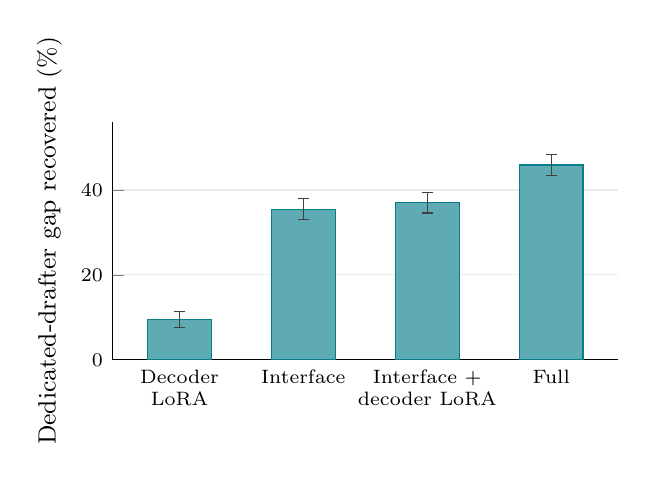
\begin{tikzpicture}
\begin{axis}[width=8.0cm,height=4.6cm,ymin=0,ymax=56,
ylabel={Dedicated-drafter gap recovered (\%)},ylabel style={font=\small},
xtick={0,1,2,3},xticklabels={Decoder\\LoRA,Interface,Interface +\\decoder LoRA,Full},
x tick label style={font=\scriptsize,align=center},tick label style={font=\scriptsize},
ymajorgrids,grid style={gray!15},axis x line*=bottom,axis y line*=left,enlarge x limits=.18]
\addplot+[ybar,mark=none,bar width=23pt,fill=teal!65,draw=teal,error bars/.cd,y dir=both,y explicit,error bar style={black!75}] coordinates {
(0,9.559455) +=(0,1.770610) -=(0,1.907351)
(1,35.499529) +=(0,2.395255) -=(0,2.401267)
(2,36.984510) +=(0,2.337847) -=(0,2.401288)
(3,45.901913) +=(0,2.418421) -=(0,2.454879)
};
\end{axis}
\end{tikzpicture}

\caption{\textbf{Where to repair.} R1 gap recovery at a matched small budget: 256 self-elicited examples, 300 steps, one seed, RedHat EAGLE-3 initialization, SPEED-128. Interface repair preserves the decoder yet captures much of full repair's gain. Bars show paired 95\% intervals; all component variants appear in Appendix~\ref{app:ablations}.}
\label{fig:components}
\end{figure}

\subsection{From acceptance to measured speed}
Figure~\ref{fig:timing} evaluates the repaired drafters against target-only generation. On R1 at batch one, interface and full repair achieve warm panel speedups of $1.74\times$ $\ci{1.58}{1.89}$ and $1.83\times$ $\ci{1.65}{1.99}$, compared with $1.31\times$ for reuse. Full repair is $1.39\times$ faster than reuse itself. On Nemotron, the repaired speedups are $1.69\times$ and $1.80\times$. At batch eight, they remain positive: $1.27\times$ and $1.29\times$ for R1, and $1.39\times$ and $1.42\times$ for Nemotron.

An independent 1B drafter offers competitive acceptance, including $\tau=2.966$ on R1 MATH-500 and higher SPEED acceptance length than the repaired family drafter on Nemotron. Its draft computation is different, however. On the batch-one timing panel it achieves $1.26\times$ for R1 and $1.37\times$ for Nemotron. This is why we evaluate wall-clock speed directly rather than interpret acceptance length as speedup. Repair retains the lightweight target-conditioned architecture while improving its proposals.

The measured seed-0 cost of 16k R1 repair is 8.92 A40 GPU-hours for response generation plus 2.21 GPU-hours for either training scope, approximately 11.12 GPU-hours per alternative. For Nemotron, the totals are 9.83 and 9.99 GPU-hours. Data generation dominates these totals and can be shared across repair variants. Interface repair's advantage here is smaller trainable state, not a demonstrated reduction in end-to-end training time. Full repair provides additional acceptance for almost the same measured R1 compute budget.

\begin{figure*}[t]
\centering
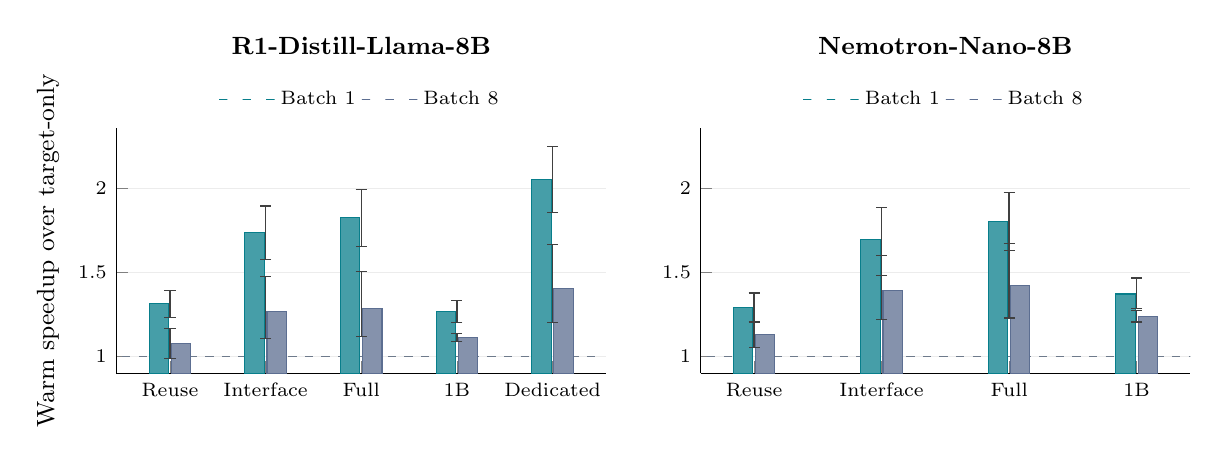
\begin{tikzpicture}
\begin{groupplot}[group style={group size=2 by 1,horizontal sep=1.2cm},
width=7.8cm,height=4.7cm,ymin=.9,ymax=2.36,ytick={1,1.5,2},
axis x line*=bottom,axis y line*=left,ymajorgrids,grid style={gray!15},
tick label style={font=\scriptsize},title style={font=\small\bfseries},
ylabel style={font=\small},enlarge x limits=.14,
legend style={draw=none,font=\scriptsize,legend columns=2,at={(.5,1.03)},anchor=south}]
\nextgroupplot[title={R1-Distill-Llama-8B},title style={yshift=17pt},xtick={0,1,2,3,4},xticklabels={Reuse,Interface,Full,1B,Dedicated},ylabel={Warm speedup over target-only}]
\draw[dashed,ink!65] (axis cs:-.5,1)--(axis cs:4.5,1);
\addplot+[ybar,bar width=7pt,bar shift=-4pt,mark=none,fill=teal!75,draw=teal,error bars/.cd,y dir=both,y explicit,error bar style={black!75,line width=.5pt}] coordinates {(0,1.312097) +=(0,0.081198) -=(0,0.081904) (1,1.737982) +=(0,0.156231) -=(0,0.160637) (2,1.828222) +=(0,0.163550) -=(0,0.176441) (3,1.264336) +=(0,0.067092) -=(0,0.063023) (4,2.054149) +=(0,0.194369) -=(0,0.199281)};
\addlegendentry{Batch 1}
\addplot+[ybar,bar width=7pt,bar shift=4pt,mark=none,fill=bluegray!75,draw=bluegray,error bars/.cd,y dir=both,y explicit,error bar style={black!75,line width=.5pt}] coordinates {(0,1.074521) +=(0,0.093352) -=(0,0.085626) (1,1.267899) +=(0,0.204759) -=(0,0.163473) (2,1.286642) +=(0,0.218616) -=(0,0.169634) (3,1.111437) +=(0,0.024409) -=(0,0.021926) (4,1.405982) +=(0,0.259471) -=(0,0.202670)};
\addlegendentry{Batch 8}
\nextgroupplot[title={Nemotron-Nano-8B},title style={yshift=17pt},xtick={0,1,2,3},xticklabels={Reuse,Interface,Full,1B}]
\draw[dashed,ink!65] (axis cs:-.5,1)--(axis cs:3.5,1);
\addplot+[ybar,bar width=7pt,bar shift=-4pt,mark=none,fill=teal!75,draw=teal,error bars/.cd,y dir=both,y explicit,error bar style={black!75,line width=.5pt}] coordinates {(0,1.291319) +=(0,0.085148) -=(0,0.087604) (1,1.693920) +=(0,0.192657) -=(0,0.211138) (2,1.802735) +=(0,0.173824) -=(0,0.174087) (3,1.370423) +=(0,0.095275) -=(0,0.085817)};
\addlegendentry{Batch 1}
\addplot+[ybar,bar width=7pt,bar shift=4pt,mark=none,fill=bluegray!75,draw=bluegray,error bars/.cd,y dir=both,y explicit,error bar style={black!75,line width=.5pt}] coordinates {(0,1.129317) +=(0,0.074756) -=(0,0.074279) (1,1.392836) +=(0,0.206947) -=(0,0.174599) (2,1.423643) +=(0,0.246541) -=(0,0.195452) (3,1.238149) +=(0,0.034481) -=(0,0.034197)};
\addlegendentry{Batch 8}
\end{groupplot}
\end{tikzpicture}

\caption{\textbf{Repair yields measured speedups.} Warm panel-time speedup over target-only decoding on A40, with paired 95\% CIs. Each arm uses three processes and three warm passes per process; batch one has 32 queries and batch eight has 128. Repair uses seed~0 and 16k target-generated responses. ``1B'' denotes the independent drafter; ``dedicated'' is available only for R1. The horizontal line is target-only speed. Startup-inclusive and token-throughput results are in Appendix~\ref{app:timing}.}
\label{fig:timing}
\end{figure*}

\subsection{Beyond one drafter architecture}
DFlash provides a second test of interface repair. With 256 self-elicited examples and 300 steps, its interface update improves SPEED first-position acceptance by 6.9 percentage points on R1 and 6.8 points on Nemotron. The corresponding paired $\Delta\tau$ values are 0.147 $\ci{0.114}{0.183}$ and 0.156 $\ci{0.117}{0.193}$. Full DFlash repair improves them to 0.235 and 0.273. These are single-seed pilots at DFlash's native $K=10$, not budget-matched comparisons against the 16k EAGLE results. They show that the repair location is useful in both an autoregressive and a block-diffusion drafter.

Repair can also be preceded by a small direct compatibility check. On the 21-checkpoint study panel, retention measured on 16 fixed queries ranks degradation on the remaining 112 queries with AUROC 1.00 $\ci{0.75}{1.00}$ for EAGLE-3 and 0.945 $\ci{0.731}{1.000}$ for DFlash. This retrospective result supports measuring compatibility before committing repair compute. Appendix~\ref{app:probe} details the fixed split and separates ranking from thresholded repair decisions.

\section{Related Work}
Speculative decoding separates token proposal from target verification \citep{leviathan2023,chen2023}. EAGLE introduces target-feature conditioning, and EAGLE-3 combines multiple target layers with training-time multi-step drafting \citep{eagle2024,eagle32025}. DFlash predicts blocks in parallel using a diffusion-style drafter \citep{dflash2026}. Recent architectural work includes H-Spec's hybrid context injection and EAGLE~3.1's normalization for draft stability \citep{hspec2026,eagle312026}. \method{} operates on already released EAGLE-3 and DFlash architectures and changes their parameters after a target update.

Draft adaptation itself is an active research direction. Domain-specific draft training studies the effect of specialization and training choices \citep{domain2025}. EDA combines a shared--private draft architecture, target-generated supervision, and representation-based data selection for fine-tuned targets \citep{eda2026}. FlexSpec addresses evolving targets in edge--cloud deployments through its model-sharing design \citep{flexspec2026}. Our emphasis is the existing target-feature projection: we localize repair without adding shared--private experts, changing the draft architecture, or requiring the original target-training examples. We evaluate that choice against full warm-start repair at matched budgets and report measured serving speed as well as acceptance.

Other approaches adapt to the states or tokens encountered during inference. Draft-OPD distills on draft-induced errors exposed by verification \citep{draftopd2026}; EvoSpec combines vocabulary adaptation with lightweight online parameter updates \citep{evospec2026}. These approaches change the training-state distribution or adapt during serving. Our experiments retain the native EAGLE-3 or DFlash objective and vocabulary, isolating the effect of repair scope after a target-model change. LoRA \citep{lora2021} supplies a useful component control, while Magpie \citep{magpie2024} supplies one way to obtain queries without the target's original corpus. The central empirical question is how much of a released drafter's capability can be retained by learning a new interface to the target.

\section{Conclusion}
A target-conditioned drafter is coupled to both the policy and the representations of its target. After post-training, that coupling can be repaired without replacing the target or redesigning the drafter. \method{} uses the target's own responses to refit the existing feature projection, recovering 59.9\% of the dedicated-drafter gap on R1 with 11.9\% of full repair's trainable parameters. Full warm-start repair raises recovery to 71.7\%. Paired results on two reasoning targets, a second drafter architecture, and measured A40 speedups establish a practical path for reusing speculative decoding as target models change.

\section*{Limitations}
The main repair results concern two 8B Llama-family targets, with three seeds for R1 and one for Nemotron; the DFlash extension uses a smaller single-seed budget. The typed population is a convenience sample, and class differences are descriptive rather than causal estimates of a post-training algorithm. Measurements use greedy decoding and a 512-token ceiling on A40 GPUs. They do not establish the same gains for unrestricted reasoning lengths, stochastic sampling, other hardware, or unseen model families. The compatibility probe is retrospective, without held-out-checkpoint validation. These scopes identify the conditions under which the reported repair and speed results were measured.

\section*{Ethical Considerations}
Repair leaves target weights and verification rules unchanged and is intended to reduce the computational cost of serving existing models. It does not improve the target's factuality or safety behavior. We use public checkpoints and prompt sources under their recorded licenses, exclude evaluation queries from repair data, and retain target-generated responses rather than filtering for favorable outcomes. No human-subject study or private user data is involved.

\bibliography{references}

\clearpage
\appendix
\section{Protocol and Reproducibility}
\label{app:protocol}
All online acceptance tables use vLLM 0.31.0 and the same frozen evaluation harness, with greedy decoding, seed~0 for generation, batch eight, a 512-token output ceiling, and NVIDIA A40 GPUs. EAGLE-3 uses $K=4$. The Llama DFlash extension uses its native $K=10$; population comparisons use $K=10$ for Llama and $K=16$ for Qwen3. Each comparison shares the exact target-rendered prompt token IDs. The reference target receives those same IDs, including the new target's template. Model snapshots, prompt hashes, per-query records, raw speculative counters, and analysis-source hashes are retained with each experiment.

Our main family drafter is \nolinkurl{yuhuili/EAGLE3-LLaMA3.1-Instruct-8B}. The dedicated R1 reference is \nolinkurl{yuhuili/EAGLE3-DeepSeek-R1-Distill-LLaMA-8B}. The second family initialization is the RedHat EAGLE-3 release for Llama-3.1-Instruct. Main targets are \nolinkurl{deepseek-ai/DeepSeek-R1-Distill-Llama-8B} and \nolinkurl{nvidia/Llama-3.1-Nemotron-Nano-8B-v1}; the independent drafter is \nolinkurl{meta-llama/Llama-3.2-1B-Instruct}. Every model is loaded from its pinned local snapshot. Licenses and model-card evidence are retained in the experiment manifests.

The 16k repair experiments use AdamW with learning rate $2\times10^{-5}$, weight decay 0.01, a cosine schedule, 3\% warmup, and a 2,048-token packed-batch ceiling. EAGLE-3 uses three native training-time-test steps with equal step weighting. The three R1 seeds are 0, 1, and 2; packing gives 4,477, 4,472, and 4,481 optimization steps, respectively. Within each seed, the paired interface/full and official/second-initialization comparisons use matched data and step budgets. The target runs in bfloat16 and receives no gradients.

The full repair scope contains the interface, draft decoder, output head, and trainable draft normalization, but excludes the frozen token embedding and target-owned verifier components. Interface repair trains only the bias-free projection in Equation~\ref{eq:interface}. Checkpoint loading follows the serving model's embedding ownership: when a release omits the embedding, the target supplies it. Trainable-parameter counts are 50,331,648 and 424,689,664. All exports retain the released vocabulary mapping and are evaluated through the same frozen serving harness.

We deduplicate repair queries against all reserved evaluation prompts, including the full 500 MATH problems. Every new generation path receives inspection of five decoded examples and answer masks. Training answers are target-generated, with the same 512-token ceiling used for data generation. The query pool changes the distribution of supervision but never introduces held-out evaluation questions. The 16k main corpus uses instruction/input fields from Alpaca (CC BY-NC 4.0), with its supplied responses discarded; small component experiments use self-elicited queries. We preserve this distinction in every comparison.

The two family initializations were compared using their paired repair gains at 16k, with SPEED as the primary panel and MATH-64 as the secondary panel. The official release had the larger gain for both update scopes and supplies the main table. This is a descriptive, data-dependent choice; the reported bootstrap intervals are not adjusted for that selection. The second release and its own reuse baseline remain in Table~\ref{tab:robustness}.

\section{Additional Acceptance Results}
\label{app:acceptance}
\begin{table*}[t]
\centering\small
\setlength{\tabcolsep}{5pt}
\begin{tabular}{@{}lllcccc@{}}
\toprule
Panel & Initialization & Scope & $p_1$ (\%) & $\tau$ & $\Delta\tau$ & Recovery (\%) \\
\midrule
SPEED & Official & Interface & \stat{62.6}{60.0--65.0} & \stat{2.414}{2.339--2.487} & \stat{0.650}{0.607--0.692} & \stat{59.9}{57.6--62.4} \\[2pt]
SPEED & Official & Full & \stat{65.0}{62.3--67.4} & \stat{2.542}{2.462--2.618} & \stat{0.778}{0.731--0.823} & \stat{71.7}{69.2--74.3} \\[2pt]
SPEED & Second release & Interface & \stat{60.6}{58.2--62.8} & \stat{2.300}{2.237--2.360} & \stat{0.569}{0.534--0.601} & \stat{50.9}{48.8--53.0} \\[2pt]
SPEED & Second release & Full & \stat{63.9}{61.4--66.2} & \stat{2.466}{2.394--2.536} & \stat{0.735}{0.693--0.776} & \stat{65.8}{63.4--68.2} \\[2pt]
MATH-64 & Official & Interface & \stat{73.3}{72.3--74.4} & \stat{2.817}{2.764--2.871} & \stat{0.894}{0.854--0.934} & \stat{45.1}{43.1--47.1} \\[2pt]
MATH-64 & Official & Full & \stat{76.0}{74.8--77.1} & \stat{2.998}{2.941--3.057} & \stat{1.074}{1.027--1.123} & \stat{54.2}{51.9--56.6} \\[2pt]
MATH-64 & Second release & Interface & \stat{70.5}{69.5--71.6} & \stat{2.658}{2.610--2.708} & \stat{0.710}{0.673--0.752} & \stat{36.3}{34.3--38.4} \\[2pt]
MATH-64 & Second release & Full & \stat{74.5}{73.5--75.4} & \stat{2.892}{2.842--2.946} & \stat{0.945}{0.901--0.988} & \stat{48.3}{46.3--50.3} \\[2pt]
\bottomrule
\end{tabular}

\caption{\textbf{Three-seed robustness on R1.} Each repair uses 16k generic queries and one epoch. Retention recovery and $\Delta\tau$ always reference the same release's reuse. The two releases are compared with paired training seeds and queries; 95\% CIs are shown. This table's MATH panel has 64 queries, unlike the seed-0 MATH-500 panel in the main table.}
\label{tab:robustness}
\end{table*}

Table~\ref{tab:robustness} reports both family initializations on both three-seed panels. The official-versus-second-release differences in repair gain on SPEED are 0.081 $\ci{0.048}{0.115}$ for interface repair and 0.043 $\ci{0.014}{0.073}$ for full repair. These contrasts subtract each initialization's own reuse before comparing repairs. Comparing repaired acceptance directly would conflate initialization quality with the benefit of repair.

The dedicated drafter is a reference point for attainable acceptance with a separately trained model. Its training data, total optimization budget, and initialization differ from the repair experiments. Consequently, gap recovery is an interpretable acceptance ratio, not a controlled estimate of how much of the dedicated model's training compute can be saved. We report measured repair cost directly rather than assign an unobserved training bill to the dedicated release.

Table~\ref{tab:depth} reports per-depth conditional acceptance and lengths on SPEED-128. Deeper positions are conditioned on the preceding accepted prefix and on a proposal being present. These rates therefore describe the surviving draft trajectories, rather than four independently sampled token positions. The main $p_1$ and $\tau$ values are query-macro statistics; pooling all speculative iterations across queries would give longer outputs greater weight.

\begin{table*}[t]
\centering\small
\begin{tabular}{@{}llccccc@{}}
\toprule
Target & Scope & $p_1$ & $p_2$ & $p_3$ & $p_4$ & Output tokens \\
\midrule
R1 & Reuse & \stat{43.0}{41.1--44.7} & \stat{42.4}{40.6--44.1} & \stat{45.8}{43.4--48.2} & \stat{50.6}{47.9--53.2} & \stat{500.906}{492.555--507.625} \\[2pt]
R1 & Interface & \stat{62.6}{59.9--65.0} & \stat{60.0}{57.8--62.0} & \stat{59.8}{57.6--61.8} & \stat{60.5}{58.2--62.6} & \stat{503.078}{497.187--508.117} \\[2pt]
R1 & Full & \stat{65.0}{62.3--67.4} & \stat{63.5}{61.4--65.4} & \stat{64.0}{62.0--65.9} & \stat{62.4}{60.1--64.5} & \stat{499.820}{492.497--505.688} \\[2pt]
Nemotron & Reuse & \stat{42.9}{40.8--45.0} & \stat{42.6}{40.3--45.0} & \stat{43.3}{40.6--46.0} & \stat{46.1}{42.3--49.8} & \stat{350.156}{321.297--378.001} \\[2pt]
Nemotron & Interface & \stat{61.4}{58.5--64.0} & \stat{61.6}{59.4--63.6} & \stat{60.5}{57.9--62.9} & \stat{64.1}{61.0--67.0} & \stat{356.211}{326.560--384.821} \\[2pt]
Nemotron & Full & \stat{62.9}{59.7--65.8} & \stat{63.1}{60.9--65.3} & \stat{61.8}{59.2--64.2} & \stat{63.8}{60.8--66.6} & \stat{352.500}{322.873--381.165} \\[2pt]
\bottomrule
\end{tabular}

\caption{\textbf{Conditional depth and output length on SPEED-128.} Percentages are query-macro conditional acceptance. R1 repair rows average three seeds; Nemotron rows use one. Brackets show 95\% query-and-seed bootstrap intervals (paired across repair and reuse). Length counts generated tokens under the 512-token ceiling.}
\label{tab:depth}
\end{table*}

\section{Component and Data Comparisons}
\label{app:ablations}
\begin{table*}[t]
\centering\small
\begin{tabular}{@{}lccc@{}}
\toprule
Updated component & $p_1$ (\%) & $\tau$ & Gap recovered (\%) \\
\midrule
RMS calibration & \stat{40.5}{38.8--42.2} & \stat{1.72}{1.68--1.77} & \stat{-0.7}{-1.6--0.2} \\[2pt]
Interface & \stat{56.4}{54.2--58.4} & \stat{2.13}{2.07--2.18} & \stat{35.5}{33.1--37.9} \\[2pt]
Interface LoRA, rank 8 & \stat{44.2}{42.4--45.9} & \stat{1.79}{1.75--1.83} & \stat{5.3}{3.1--7.4} \\[2pt]
Interface LoRA, rank 32 & \stat{48.5}{46.5--50.3} & \stat{1.90}{1.85--1.95} & \stat{15.4}{13.1--17.4} \\[2pt]
Decoder LoRA & \stat{45.6}{43.7--47.3} & \stat{1.84}{1.79--1.88} & \stat{9.6}{7.7--11.3} \\[2pt]
Interface + decoder LoRA & \stat{56.6}{54.3--58.7} & \stat{2.14}{2.09--2.20} & \stat{37.0}{34.6--39.3} \\[2pt]
Full warm start & \stat{58.7}{56.3--60.8} & \stat{2.24}{2.18--2.30} & \stat{45.9}{43.4--48.3} \\[2pt]
Scratch draft layers/head & \stat{16.7}{15.8--17.6} & \stat{1.21}{1.19--1.22} & \stat{-46.7}{-50.9---43.0} \\[2pt]
\bottomrule
\end{tabular}

\caption{\textbf{Complete small-budget component comparison.} R1-Llama, RedHat family initialization, 256 self-elicited examples, 300 training steps, one seed, SPEED-128, $K=4$. Calibration is training-free and fitted on a separate 256-example path; it is not a 300-step optimizer run. Intervals are paired query bootstrap intervals. Decoder LoRA is an update-scope control, not a reproduction of EDA.}
\label{tab:components}
\end{table*}

Table~\ref{tab:components} retains the complete small-budget component comparison. Low-rank updates to the interface use ranks 8 and 32. Decoder LoRA updates query/value attention projections and MLP projections while holding the interface fixed. The combined variant updates the interface and these decoder adapters. Adapters are merged before evaluation. Random initialization resets the trainable interface, draft layers, head, and normalization while retaining fixed embeddings and the vocabulary map; it does not retrain the target.

The full interface update outperforms the lower-rank interface controls at this budget. This distinguishes the location of repair from a claim that arbitrarily low-rank repair suffices. Likewise, the decoder-only control is weaker than interface repair, while combining the two is close to the interface result. These comparisons support a useful repair location without establishing that one component is the unique source of drift.

Training-free moment calibration provides another control. We fit per-layer mean/RMS affine transformations on paired parent/target forwards. Full affine correction is an offline teacher-forced diagnostic because the frozen serving projection is bias-free; RMS-only correction can be exported exactly. On 64 held-out target-generated R1 contexts, full affine calibration changes agreement with the target verifier by $-0.15$ percentage points $\ci{-0.31}{0.01}$. RMS-only changes it by $-0.22$ points $\ci{-0.37}{-0.08}$. Thus the learned interface result is not reproduced by this scalar moment correction.

\begin{table}[t]
\centering\small
\begin{tabular}{@{}lcc@{}}
\toprule
Queries & Interface $\tau$ & Full $\tau$ \\
\midrule
Self-elicited 256 & \stat{2.127}{2.071--2.181} & \stat{2.243}{2.181--2.303} \\[2pt]
Self-elicited 1k & \stat{2.137}{2.078--2.193} & \stat{2.261}{2.198--2.322} \\[2pt]
Self-elicited 4k & \stat{2.220}{2.156--2.280} & \stat{2.365}{2.295--2.432} \\[2pt]
Generic 4k & \stat{2.224}{2.162--2.282} & \stat{2.374}{2.305--2.440} \\[2pt]
Generic 16k & \stat{2.294}{2.228--2.357} & \stat{2.459}{2.386--2.529} \\[2pt]
\bottomrule
\end{tabular}

\caption{\textbf{Query source and scale.} R1 SPEED-128 acceptance length with the second family initialization, seed~0. The 256-example runs use 300 steps; the 1k/4k/16k runs use one epoch. Generic and self-elicited corpora have different token counts, so source comparisons are matched by examples and epoch rather than token budget. All rows use target-generated answers.}
\label{tab:scaling}
\end{table}

Table~\ref{tab:scaling} separates data scale from query source. At 4k, generic and self-elicited queries give similar final acceptance: interface $\tau$ is 2.224 versus 2.220, and full repair is 2.374 versus 2.365. We therefore use the generic public pool for the larger main experiment without attributing the repair gains to a unique prompt-generation strategy. Increasing the generic pool to 16k raises seed-0 $\tau$ to 2.294 and 2.459 with the second initialization; Table~\ref{tab:robustness} reports the three-seed averages.

A matched 16k scratch run reaches $\tau=1.519$ on SPEED and is distinct from the 256-example scratch row. A second epoch of full warm-start training reaches 2.480, while increasing the native training unroll from three to four steps at generic-4k yields 2.220 for the interface and 2.367 for full repair. We keep the three-step, one-epoch setting for the main comparison. These controls characterize the chosen operating point rather than supply additional independent replications.

\section{DFlash Extension}
\label{app:dflash}
\begin{table*}[t]
\centering\small
\begin{tabular}{@{}llcccc@{}}
\toprule
Target & Repair & SPEED $\Delta p_1$ (pp) & SPEED $\Delta\tau$ & MATH $\Delta p_1$ (pp) & MATH $\Delta\tau$ \\
\midrule
R1 & Interface & 6.86 [6.08,7.67] & .147 [.114,.183] & 5.90 [4.75,7.03] & .177 [.128,.227] \\
R1 & Full & 10.03 [9.18,10.86] & .235 [.195,.269] & 9.02 [7.81,10.21] & .258 [.211,.304] \\
Nemotron & Interface & 6.81 [5.87,7.79] & .156 [.117,.193] & 6.86 [6.03,7.69] & .175 [.155,.196] \\
Nemotron & Full & 9.70 [8.61,10.80] & .273 [.225,.322] & 11.42 [10.52,12.33] & .329 [.298,.361] \\
\bottomrule
\end{tabular}
\caption{\textbf{DFlash repair pilot.} Paired changes over DFlash's own reuse; 256 self-elicited examples per target, 300 steps, one seed, native $K=10$, SPEED-128 and MATH-64. Intervals use 10,000 paired query resamples. No EAGLE dedicated reference is used to compute DFlash recovery.}
\label{tab:dflash}
\end{table*}

DFlash uses native block KL training, 64 anchors, decay parameter four, and fixed exponential position weighting. Both scopes use learning rate $2\times10^{-5}$, the 2,048-token ceiling, a 300-step cosine schedule, 3\% warmup, and weight decay 0.01. The interface has 83,886,080 trainable parameters; the full scope has 1,048,626,432. Verifier-owned full-vocabulary components remain fixed.

At 300 steps, interface and full repair improve both $p_1$ and $\tau$ on both targets and workloads (Table~\ref{tab:dflash}). Measured data-plus-training costs are 0.391/0.430 A40 GPU-hours for R1 interface/full and 0.294/0.338 for Nemotron. Those costs use a much smaller corpus and budget than the EAGLE flagship experiment. The extension tests whether the same repair location remains useful under another native architecture and loss, not a causal architecture comparison at equal compute.

\section{Timing and Cost}
\label{app:timing}
\begin{table*}[t]
\centering\small
\setlength{\tabcolsep}{4pt}
\begin{tabular}{@{}llccc@{}}
\toprule
Target / batch & Drafter & Warm speedup & Token throughput & Startup inclusive \\
\midrule
R1 / 1 & Reuse family drafter & 1.31 [1.23, 1.39] & 1.32 [1.25, 1.39] & 1.15 [1.10, 1.20] \\
R1 / 1 & ReFit--interface & 1.74 [1.58, 1.89] & 1.75 [1.59, 1.90] & 1.40 [1.31, 1.49] \\
R1 / 1 & ReFit--full & 1.83 [1.65, 1.99] & 1.84 [1.67, 2.00] & 1.46 [1.36, 1.55] \\
R1 / 1 & Independent 1B drafter & 1.26 [1.20, 1.33] & 1.26 [1.21, 1.32] & 1.14 [1.10, 1.18] \\
R1 / 1 & Dedicated R1 drafter & 2.05 [1.85, 2.25] & 2.07 [1.88, 2.25] & 1.58 [1.47, 1.69] \\
\addlinespace[2pt]
R1 / 8 & Reuse family drafter & 1.07 [0.99, 1.17] & 1.07 [0.99, 1.16] & 0.95 [0.90, 1.01] \\
R1 / 8 & ReFit--interface & 1.27 [1.10, 1.47] & 1.27 [1.10, 1.47] & 1.07 [0.98, 1.19] \\
R1 / 8 & ReFit--full & 1.29 [1.12, 1.51] & 1.28 [1.11, 1.50] & 1.09 [0.99, 1.21] \\
R1 / 8 & Independent 1B drafter & 1.11 [1.09, 1.14] & 1.11 [1.09, 1.13] & 0.99 [0.95, 1.03] \\
R1 / 8 & Dedicated R1 drafter & 1.41 [1.20, 1.67] & 1.40 [1.20, 1.66] & 1.11 [1.00, 1.22] \\
\addlinespace[2pt]
Nemotron / 1 & Reuse family drafter & 1.29 [1.20, 1.38] & 1.31 [1.24, 1.37] & 1.17 [1.07, 1.31] \\
Nemotron / 1 & ReFit--interface & 1.69 [1.48, 1.89] & 1.74 [1.59, 1.88] & 1.42 [1.27, 1.59] \\
Nemotron / 1 & ReFit--full & 1.80 [1.63, 1.98] & 1.82 [1.65, 1.99] & 1.48 [1.35, 1.65] \\
Nemotron / 1 & Independent 1B drafter & 1.37 [1.28, 1.47] & 1.38 [1.31, 1.46] & 1.22 [1.12, 1.36] \\
\addlinespace[2pt]
Nemotron / 8 & Reuse family drafter & 1.13 [1.06, 1.20] & 1.13 [1.05, 1.21] & 0.97 [0.92, 1.01] \\
Nemotron / 8 & ReFit--interface & 1.39 [1.22, 1.60] & 1.38 [1.21, 1.59] & 1.11 [1.02, 1.22] \\
Nemotron / 8 & ReFit--full & 1.42 [1.23, 1.67] & 1.42 [1.23, 1.66] & 1.16 [1.05, 1.29] \\
Nemotron / 8 & Independent 1B drafter & 1.24 [1.20, 1.27] & 1.23 [1.19, 1.27] & 1.09 [1.05, 1.13] \\
\addlinespace[2pt]
\bottomrule
\end{tabular}

\caption{\textbf{Measured A40 timing.} All ratios are relative to target-only decoding on paired query panels. Warm results average three passes within each of three processes. Startup-inclusive results charge engine loading/compilation plus the first panel. Batch one uses 32 queries, batch eight 128. Intervals jointly resample process pairs and query batches.}
\label{tab:timing}
\end{table*}

Timing uses a fixed query panel and fresh controls within the same measurement wave. A process performs one cold panel followed by three warm passes. Warm speedup is the target-only panel time divided by speculative panel time, after averaging warm passes within process. We also report the ratio of generated-token throughput and the first-panel ratio including engine startup. The seed-0 checkpoints are used for timing; repeated processes are serving repetitions, not additional training seeds.

Queries are paired across arms, but execution uses available A40 hosts rather than randomized exclusive-host allocation. Greedy outputs can differ across serving configurations, so the timing estimand is the runtime of the same query workload rather than an identical sequence of output tokens. Token-throughput ratios and generated lengths are retained to make this distinction visible. On R1 at batch one, full repair's panel speedup is 1.83 and token-throughput ratio 1.84; the startup-inclusive ratio is 1.46. These are different deployment costs and should not be interchanged.

\begin{table}[t]
\centering\small
\begin{tabular}{@{}llrrr@{}}
\toprule
Target & Scope & Data & Train & Total \\
\midrule
R1 & Interface & 8.916 & 2.206 & 11.122 \\
R1 & Full & 8.916 & 2.211 & 11.127 \\
Nemotron & Interface & 8.588 & 1.240 & 9.828 \\
Nemotron & Full & 8.588 & 1.398 & 9.986 \\
\bottomrule
\end{tabular}
\caption{\textbf{Measured repair GPU-hours.} A40, 16k examples, seed~0. Each alternative is charged the shared data-generation cost once. Totals exclude evaluation, engineering, and the broader experimental search.}
\label{tab:cost}
\end{table}

\section{Population and Diagnostic Scope}
\label{app:population}
The model-card inventory contains 201 records: the historical 174-checkpoint census, 18 target-conditioned candidates, eight expansion checkpoints, and one additional candidate. Forty-five training histories remain unknown. Labels record checkpoint-specific evidence where available and keep lineage separate from cumulative training history. R1-Llama and R1-Qwen are siblings of the family drafter's instruction target, rather than direct children. Nemotron's combined SFT/RL/merge history is not entered into the pure on-policy RL group.

The focused frozen-harness panel contains 25 checkpoints before filters. Two are pretrained controls and two were flagged as collapsed checkpoints; they remain separate from the 21-checkpoint post-training summary. Two additional candidate repositories have incompatible architecture and do not enter valid pairs. The 21 retained checkpoints contribute 42 SPEED comparisons, and eight of them also contribute 16 MATH comparisons. Figure~\ref{fig:retention} shows only groups with multiple checkpoints. Its intervals resample checkpoints and then paired query IDs; related checkpoints can still share a training trajectory. The historical census is provenance-distinct and is not silently pooled into this panel.

The fixed-prefix diagnostic uses 64 sequences for each of five targets and three text origins: saved parent completions, saved target completions, and public MATH reference solutions. Within a sequence, all feature-source/verifier combinations share exact prefix tokens. Comparisons across origins also change the questions and lengths, and therefore are not treated as controlled effects of text origin. We use full-vocabulary verifier argmax, retaining out-of-draft-support tokens as disagreement rather than renormalizing the greedy answer into support.

R1-Qwen shows negative feature-source and policy effects on target-generated contexts, like the two flagship targets. The T\"ulu DPO feature effect is near zero, while its policy effect is negative; the Qwen GRPO control is near zero on both. This is consistent with treating the interface as a useful repair location rather than a universal, exclusive explanation of every acceptance loss. A same-weight Nemotron reasoning toggle changes EAGLE $p_1$ by $-2.96$ points $\ci{-4.37}{-1.57}$ and DFlash by $-2.78$ points on the paired raw-query panel. Context and policy changes can therefore contribute alongside feature-source changes.

\section{Retrospective Compatibility Probe}
\label{app:probe}
We choose two SPEED batch indices by a fixed hash rule, yielding 16 probe queries, and use the remaining 112 to label degradation as $p_1$ retention below 0.9. The split is shared across all 21 eligible checkpoints and both drafters. No model is trained and no cutoff is optimized. One immediate-EOS query has no acceptance opportunities and is excluded pairwise where necessary.

The full 16-query probe achieves EAGLE AUROC 1.00 with a checkpoint-and-query interval $\ci{0.75}{1.00}$, and DFlash AUROC 0.945 $\ci{0.731}{1.000}$. At the fixed 0.9 decision cutoff, EAGLE has seven true positives, three false positives, no false negatives, and 11 true negatives; DFlash has nine, three, one, and eight. Thus ranking a small cohort is different from making error-free repair decisions. The evaluation is retrospective and does not hold out checkpoint lineages.

Captured generation times for the full request subset, summing both target arms, have medians 45.2 seconds for EAGLE and 39.3 seconds for DFlash; separate engine startups add median totals of 274.7 and 302.4 seconds. These are observed request costs, not a sub-minute cold deployment claim. Restricting the probe to the first 16 speculative iterations lowers the EAGLE AUROC to 0.602 and DFlash to 0.773. The complete request measurement supports compatibility triage, while very short prefixes are not a substitute for the measured panel.

\end{document}
